\documentclass[1p]{elsarticle_modified}
%\bibliographystyle{elsarticle-num}

%\usepackage[colorlinks]{hyperref}
%\usepackage{abbrmath_seonhwa} %\Abb, \Ascr, \Acal ,\Abf, \Afrak
\usepackage{amsfonts}
\usepackage{amssymb}
\usepackage{amsmath}
\usepackage{amsthm}
\usepackage{scalefnt}
\usepackage{amsbsy}
\usepackage{kotex}
\usepackage{caption}
\usepackage{subfig}
\usepackage{color}
\usepackage{graphicx}
\usepackage{xcolor} %% white, black, red, green, blue, cyan, magenta, yellow
\usepackage{float}
\usepackage{setspace}
\usepackage{hyperref}

\usepackage{tikz}
\usetikzlibrary{arrows}

\usepackage{multirow}
\usepackage{array} % fixed length table
\usepackage{hhline}

%%%%%%%%%%%%%%%%%%%%%
\makeatletter
\renewcommand*\env@matrix[1][\arraystretch]{%
	\edef\arraystretch{#1}%
	\hskip -\arraycolsep
	\let\@ifnextchar\new@ifnextchar
	\array{*\c@MaxMatrixCols c}}
\makeatother %https://tex.stackexchange.com/questions/14071/how-can-i-increase-the-line-spacing-in-a-matrix
%%%%%%%%%%%%%%%

\usepackage[normalem]{ulem}

\newcommand{\msout}[1]{\ifmmode\text{\sout{\ensuremath{#1}}}\else\sout{#1}\fi}
%SOURCE: \msout is \stkout macro in https://tex.stackexchange.com/questions/20609/strikeout-in-math-mode

\newcommand{\cancel}[1]{
	\ifmmode
	{\color{red}\msout{#1}}
	\else
	{\color{red}\sout{#1}}
	\fi
}

\newcommand{\add}[1]{
	{\color{blue}\uwave{#1}}
}

\newcommand{\replace}[2]{
	\ifmmode
	{\color{red}\msout{#1}}{\color{blue}\uwave{#2}}
	\else
	{\color{red}\sout{#1}}{\color{blue}\uwave{#2}}
	\fi
}

\newcommand{\Sol}{\mathcal{S}} %segment
\newcommand{\D}{D} %diagram
\newcommand{\A}{\mathcal{A}} %arc


%%%%%%%%%%%%%%%%%%%%%%%%%%%%%5 test

\def\sl{\operatorname{\textup{SL}}(2,\Cbb)}
\def\psl{\operatorname{\textup{PSL}}(2,\Cbb)}
\def\quan{\mkern 1mu \triangleright \mkern 1mu}

\theoremstyle{definition}
\newtheorem{thm}{Theorem}[section]
\newtheorem{prop}[thm]{Proposition}
\newtheorem{lem}[thm]{Lemma}
\newtheorem{ques}[thm]{Question}
\newtheorem{cor}[thm]{Corollary}
\newtheorem{defn}[thm]{Definition}
\newtheorem{exam}[thm]{Example}
\newtheorem{rmk}[thm]{Remark}
\newtheorem{alg}[thm]{Algorithm}

\newcommand{\I}{\sqrt{-1}}
\begin{document}

%\begin{frontmatter}
%
%\title{Boundary parabolic representations of knots up to 8 crossings}
%
%%% Group authors per affiliation:
%\author{Yunhi Cho} 
%\address{Department of Mathematics, University of Seoul, Seoul, Korea}
%\ead{yhcho@uos.ac.kr}
%
%
%\author{Seonhwa Kim} %\fnref{s_kim}}
%\address{Center for Geometry and Physics, Institute for Basic Science, Pohang, 37673, Korea}
%\ead{ryeona17@ibs.re.kr}
%
%\author{Hyuk Kim}
%\address{Department of Mathematical Sciences, Seoul National University, Seoul 08826, Korea}
%\ead{hyukkim@snu.ac.kr}
%
%\author{Seokbeom Yoon}
%\address{Department of Mathematical Sciences, Seoul National University, Seoul, 08826,  Korea}
%\ead{sbyoon15@snu.ac.kr}
%
%\begin{abstract}
%We find all boundary parabolic representation of knots up to 8 crossings.
%
%\end{abstract}
%\begin{keyword}
%    \MSC[2010] 57M25 
%\end{keyword}
%
%\end{frontmatter}

%\linenumbers
%\tableofcontents
%
\newcommand\colored[1]{\textcolor{white}{\rule[-0.35ex]{0.8em}{1.4ex}}\kern-0.8em\color{red} #1}%
%\newcommand\colored[1]{\textcolor{white}{ #1}\kern-2.17ex	\textcolor{white}{ #1}\kern-1.81ex	\textcolor{white}{ #1}\kern-2.15ex\color{red}#1	}

{\Large $\underline{12a_{0649}~(K12a_{0649})}$}

\setlength{\tabcolsep}{10pt}
\renewcommand{\arraystretch}{1.6}
\vspace{1cm}\begin{tabular}{m{100pt}>{\centering\arraybackslash}m{274pt}}
\multirow{5}{120pt}{
	\centering
	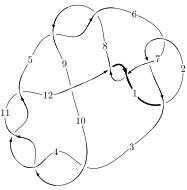
\includegraphics[width=112pt]{../../../GIT/diagram.site/Diagrams/png/1450_12a_0649.png}\\
\ \ \ A knot diagram\footnotemark}&
\allowdisplaybreaks
\textbf{Linearized knot diagam} \\
\cline{2-2}
 &
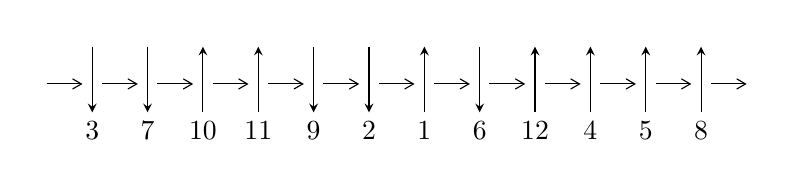
\begin{tikzpicture}[x=20pt, y=17pt]
	% nodes
	\node (C0) at (0, 0) {};
	\node (C1) at (1, 0) {};
	\node (C1U) at (1, +1) {};
	\node (C1D) at (1, -1) {3};

	\node (C2) at (2, 0) {};
	\node (C2U) at (2, +1) {};
	\node (C2D) at (2, -1) {7};

	\node (C3) at (3, 0) {};
	\node (C3U) at (3, +1) {};
	\node (C3D) at (3, -1) {10};

	\node (C4) at (4, 0) {};
	\node (C4U) at (4, +1) {};
	\node (C4D) at (4, -1) {11};

	\node (C5) at (5, 0) {};
	\node (C5U) at (5, +1) {};
	\node (C5D) at (5, -1) {9};

	\node (C6) at (6, 0) {};
	\node (C6U) at (6, +1) {};
	\node (C6D) at (6, -1) {2};

	\node (C7) at (7, 0) {};
	\node (C7U) at (7, +1) {};
	\node (C7D) at (7, -1) {1};

	\node (C8) at (8, 0) {};
	\node (C8U) at (8, +1) {};
	\node (C8D) at (8, -1) {6};

	\node (C9) at (9, 0) {};
	\node (C9U) at (9, +1) {};
	\node (C9D) at (9, -1) {12};

	\node (C10) at (10, 0) {};
	\node (C10U) at (10, +1) {};
	\node (C10D) at (10, -1) {4};

	\node (C11) at (11, 0) {};
	\node (C11U) at (11, +1) {};
	\node (C11D) at (11, -1) {5};

	\node (C12) at (12, 0) {};
	\node (C12U) at (12, +1) {};
	\node (C12D) at (12, -1) {8};
	\node (C13) at (13, 0) {};

	% arrows
	\draw[->,>={angle 60}]
	(C0) edge (C1) (C1) edge (C2) (C2) edge (C3) (C3) edge (C4) (C4) edge (C5) (C5) edge (C6) (C6) edge (C7) (C7) edge (C8) (C8) edge (C9) (C9) edge (C10) (C10) edge (C11) (C11) edge (C12) (C12) edge (C13) ;	\draw[->,>=stealth]
	(C1U) edge (C1D) (C2U) edge (C2D) (C3D) edge (C3U) (C4D) edge (C4U) (C5U) edge (C5D) (C6U) edge (C6D) (C7D) edge (C7U) (C8U) edge (C8D) (C9D) edge (C9U) (C10D) edge (C10U) (C11D) edge (C11U) (C12D) edge (C12U) ;
	\end{tikzpicture} \\
\hhline{~~} \\& 
\textbf{Solving Sequence} \\ \cline{2-2} 
 &
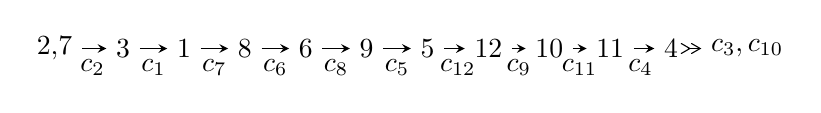
\begin{tikzpicture}[x=22pt, y=7pt]
	% node
	\node (A0) at (-1/8, 0) {2,7};
	\node (A1) at (1, 0) {3};
	\node (A2) at (2, 0) {1};
	\node (A3) at (3, 0) {8};
	\node (A4) at (4, 0) {6};
	\node (A5) at (5, 0) {9};
	\node (A6) at (6, 0) {5};
	\node (A7) at (7, 0) {12};
	\node (A8) at (8, 0) {10};
	\node (A9) at (9, 0) {11};
	\node (A10) at (10, 0) {4};
	\node (C1) at (1/2, -1) {$c_{2}$};
	\node (C2) at (3/2, -1) {$c_{1}$};
	\node (C3) at (5/2, -1) {$c_{7}$};
	\node (C4) at (7/2, -1) {$c_{6}$};
	\node (C5) at (9/2, -1) {$c_{8}$};
	\node (C6) at (11/2, -1) {$c_{5}$};
	\node (C7) at (13/2, -1) {$c_{12}$};
	\node (C8) at (15/2, -1) {$c_{9}$};
	\node (C9) at (17/2, -1) {$c_{11}$};
	\node (C10) at (19/2, -1) {$c_{4}$};
	\node (A11) at (45/4, 0) {$c_{3},c_{10}$};

	% edge
	\draw[->,>=stealth]	
	(A0) edge (A1) (A1) edge (A2) (A2) edge (A3) (A3) edge (A4) (A4) edge (A5) (A5) edge (A6) (A6) edge (A7) (A7) edge (A8) (A8) edge (A9) (A9) edge (A10) ;
	\draw[->>,>={angle 60}]	
	(A10) edge (A11);
\end{tikzpicture} \\ 

\end{tabular} \\

\footnotetext{
The image of knot diagram is generated by the software ``\textbf{Draw programme}" developed by Andrew Bartholomew(\url{http://www.layer8.co.uk/maths/draw/index.htm\#Running-draw}), where we modified some parts for our purpose(\url{https://github.com/CATsTAILs/LinksPainter}).
}\phantom \\ \newline 
\centering \textbf{Ideals for irreducible components\footnotemark of $X_{\text{par}}$} 
 
\begin{align*}
I^u_{1}&=\langle 
u^{63}+u^{62}+\cdots+2 u+1\rangle \\
\\
\end{align*}
\raggedright * 1 irreducible components of $\dim_{\mathbb{C}}=0$, with total 63 representations.\\
\footnotetext{All coefficients of polynomials are rational numbers. But the coefficients are sometimes approximated in decimal forms when there is not enough margin.}
\newpage
\renewcommand{\arraystretch}{1}
\centering \section*{I. $I^u_{1}= \langle u^{63}+u^{62}+\cdots+2 u+1 \rangle$}
\flushleft \textbf{(i) Arc colorings}\\
\begin{tabular}{m{7pt} m{180pt} m{7pt} m{180pt} }
\flushright $a_{2}=$&$\begin{pmatrix}1\\0\end{pmatrix}$ \\
\flushright $a_{7}=$&$\begin{pmatrix}0\\u\end{pmatrix}$ \\
\flushright $a_{3}=$&$\begin{pmatrix}1\\u^2\end{pmatrix}$ \\
\flushright $a_{1}=$&$\begin{pmatrix}- u^2+1\\- u^4\end{pmatrix}$ \\
\flushright $a_{8}=$&$\begin{pmatrix}u^5-2 u^3+u\\u^7- u^5+u\end{pmatrix}$ \\
\flushright $a_{6}=$&$\begin{pmatrix}u\\u\end{pmatrix}$ \\
\flushright $a_{9}=$&$\begin{pmatrix}- u^9+2 u^7- u^5-2 u^3+u\\- u^9+3 u^7-3 u^5+u\end{pmatrix}$ \\
\flushright $a_{5}=$&$\begin{pmatrix}u^{17}-4 u^{15}+7 u^{13}-4 u^{11}-3 u^9+6 u^7-2 u^5+u\\u^{17}-5 u^{15}+11 u^{13}-12 u^{11}+5 u^9+2 u^7-2 u^5+u\end{pmatrix}$ \\
\flushright $a_{12}=$&$\begin{pmatrix}- u^8+3 u^6-3 u^4+1\\- u^{10}+2 u^8- u^6-2 u^4+u^2\end{pmatrix}$ \\
\flushright $a_{10}=$&$\begin{pmatrix}u^{27}-8 u^{25}+\cdots-3 u^3+2 u\\u^{29}-7 u^{27}+\cdots+u^3+u\end{pmatrix}$ \\
\flushright $a_{11}=$&$\begin{pmatrix}u^{44}-11 u^{42}+\cdots+u^2+1\\u^{44}-12 u^{42}+\cdots-3 u^4+2 u^2\end{pmatrix}$ \\
\flushright $a_{4}=$&$\begin{pmatrix}- u^{54}+15 u^{52}+\cdots-2 u^2+1\\- u^{56}+14 u^{54}+\cdots-13 u^8+10 u^6\end{pmatrix}$\\&\end{tabular}
\flushleft \textbf{(ii) Obstruction class $= -1$}\\~\\
\flushleft \textbf{(iii) Cusp Shapes $= 4 u^{61}-64 u^{59}+\cdots-8 u+6$}\\~\\
\newpage\renewcommand{\arraystretch}{1}
\flushleft \textbf{(iv) u-Polynomials at the component}\newline \\
\begin{tabular}{m{50pt}|m{274pt}}
Crossings & \hspace{64pt}u-Polynomials at each crossing \\
\hline $$\begin{aligned}c_{1}\end{aligned}$$&$\begin{aligned}
&u^{63}+33 u^{62}+\cdots+4 u+1
\end{aligned}$\\
\hline $$\begin{aligned}c_{2},c_{6}\end{aligned}$$&$\begin{aligned}
&u^{63}- u^{62}+\cdots+2 u-1
\end{aligned}$\\
\hline $$\begin{aligned}c_{3},c_{4},c_{10}\\c_{11}\end{aligned}$$&$\begin{aligned}
&u^{63}+u^{62}+\cdots+2 u^2-1
\end{aligned}$\\
\hline $$\begin{aligned}c_{5},c_{8}\end{aligned}$$&$\begin{aligned}
&u^{63}-5 u^{62}+\cdots-384 u+41
\end{aligned}$\\
\hline $$\begin{aligned}c_{7},c_{12}\end{aligned}$$&$\begin{aligned}
&u^{63}-3 u^{62}+\cdots+164 u-9
\end{aligned}$\\
\hline $$\begin{aligned}c_{9}\end{aligned}$$&$\begin{aligned}
&u^{63}+19 u^{62}+\cdots+38968 u+4073
\end{aligned}$\\
\hline
\end{tabular}\\~\\
\newpage\renewcommand{\arraystretch}{1}
\flushleft \textbf{(v) Riley Polynomials at the component}\newline \\
\begin{tabular}{m{50pt}|m{274pt}}
Crossings & \hspace{64pt}Riley Polynomials at each crossing \\
\hline $$\begin{aligned}c_{1}\end{aligned}$$&$\begin{aligned}
&y^{63}-5 y^{62}+\cdots-8 y-1
\end{aligned}$\\
\hline $$\begin{aligned}c_{2},c_{6}\end{aligned}$$&$\begin{aligned}
&y^{63}-33 y^{62}+\cdots+4 y-1
\end{aligned}$\\
\hline $$\begin{aligned}c_{3},c_{4},c_{10}\\c_{11}\end{aligned}$$&$\begin{aligned}
&y^{63}-73 y^{62}+\cdots+4 y-1
\end{aligned}$\\
\hline $$\begin{aligned}c_{5},c_{8}\end{aligned}$$&$\begin{aligned}
&y^{63}+47 y^{62}+\cdots-36224 y-1681
\end{aligned}$\\
\hline $$\begin{aligned}c_{7},c_{12}\end{aligned}$$&$\begin{aligned}
&y^{63}+43 y^{62}+\cdots+27400 y-81
\end{aligned}$\\
\hline $$\begin{aligned}c_{9}\end{aligned}$$&$\begin{aligned}
&y^{63}-25 y^{62}+\cdots+96017920 y-16589329
\end{aligned}$\\
\hline
\end{tabular}\\~\\
\newpage\flushleft \textbf{(vi) Complex Volumes and Cusp Shapes}
$$\begin{array}{c|c|c}  
\text{Solutions to }I^u_{1}& \I (\text{vol} + \sqrt{-1}CS) & \text{Cusp shape}\\
 \hline 
\begin{aligned}
u &= -0.807336 + 0.596819 I\end{aligned}
 & \phantom{-}13.3335 + 7.7246 I & \phantom{-}10.00998 - 6.36298 I \\ \hline\begin{aligned}
u &= -0.807336 - 0.596819 I\end{aligned}
 & \phantom{-}13.3335 - 7.7246 I & \phantom{-}10.00998 + 6.36298 I \\ \hline\begin{aligned}
u &= \phantom{-}0.797322 + 0.579716 I\end{aligned}
 & \phantom{-}5.11223 - 5.63114 I & \phantom{-}8.39389 + 7.97661 I \\ \hline\begin{aligned}
u &= \phantom{-}0.797322 - 0.579716 I\end{aligned}
 & \phantom{-}5.11223 + 5.63114 I & \phantom{-}8.39389 - 7.97661 I \\ \hline\begin{aligned}
u &= -0.971710\phantom{ +0.000000I}\end{aligned}
 & \phantom{-}4.41099\phantom{ +0.000000I} & -0.384110\phantom{ +0.000000I} \\ \hline\begin{aligned}
u &= -0.924847 + 0.292781 I\end{aligned}
 & -0.45640 + 3.17636 I & \phantom{-}1.88577 - 8.75054 I \\ \hline\begin{aligned}
u &= -0.924847 - 0.292781 I\end{aligned}
 & -0.45640 - 3.17636 I & \phantom{-}1.88577 + 8.75054 I \\ \hline\begin{aligned}
u &= -0.771159 + 0.561770 I\end{aligned}
 & \phantom{-}2.89928 + 2.24328 I & \phantom{-}4.38244 - 3.59011 I \\ \hline\begin{aligned}
u &= -0.771159 - 0.561770 I\end{aligned}
 & \phantom{-}2.89928 - 2.24328 I & \phantom{-}4.38244 + 3.59011 I \\ \hline\begin{aligned}
u &= -0.734481 + 0.605389 I\end{aligned}
 & \phantom{-}13.54260 - 3.01261 I & \phantom{-}10.67968 - 0.23092 I \\ \hline\begin{aligned}
u &= -0.734481 - 0.605389 I\end{aligned}
 & \phantom{-}13.54260 + 3.01261 I & \phantom{-}10.67968 + 0.23092 I \\ \hline\begin{aligned}
u &= \phantom{-}0.961610 + 0.434304 I\end{aligned}
 & \phantom{-}7.01116 - 4.42511 I & \phantom{-}6.14172 + 6.08207 I \\ \hline\begin{aligned}
u &= \phantom{-}0.961610 - 0.434304 I\end{aligned}
 & \phantom{-}7.01116 + 4.42511 I & \phantom{-}6.14172 - 6.08207 I \\ \hline\begin{aligned}
u &= \phantom{-}0.741982 + 0.582849 I\end{aligned}
 & \phantom{-}5.27071 + 1.03217 I & \phantom{-}9.12178 - 1.02959 I \\ \hline\begin{aligned}
u &= \phantom{-}0.741982 - 0.582849 I\end{aligned}
 & \phantom{-}5.27071 - 1.03217 I & \phantom{-}9.12178 + 1.02959 I \\ \hline\begin{aligned}
u &= \phantom{-}0.858425 + 0.141613 I\end{aligned}
 & -1.43959 - 0.53362 I & -4.53498 + 0.33396 I \\ \hline\begin{aligned}
u &= \phantom{-}0.858425 - 0.141613 I\end{aligned}
 & -1.43959 + 0.53362 I & -4.53498 - 0.33396 I \\ \hline\begin{aligned}
u &= \phantom{-}1.103660 + 0.285741 I\end{aligned}
 & \phantom{-}7.32672 - 4.55583 I & \phantom{-0.000000 } 0 \\ \hline\begin{aligned}
u &= \phantom{-}1.103660 - 0.285741 I\end{aligned}
 & \phantom{-}7.32672 + 4.55583 I & \phantom{-0.000000 } 0 \\ \hline\begin{aligned}
u &= -1.114240 + 0.357197 I\end{aligned}
 & -0.73485 + 3.08669 I & \phantom{-0.000000 } 0 \\ \hline\begin{aligned}
u &= -1.114240 - 0.357197 I\end{aligned}
 & -0.73485 - 3.08669 I & \phantom{-0.000000 } 0 \\ \hline\begin{aligned}
u &= -0.200631 + 0.794151 I\end{aligned}
 & \phantom{-}10.38970 - 8.95920 I & \phantom{-}8.29474 + 4.99884 I \\ \hline\begin{aligned}
u &= -0.200631 - 0.794151 I\end{aligned}
 & \phantom{-}10.38970 + 8.95920 I & \phantom{-}8.29474 - 4.99884 I \\ \hline\begin{aligned}
u &= \phantom{-}0.193476 + 0.779461 I\end{aligned}
 & \phantom{-}2.31625 + 6.69956 I & \phantom{-}6.24548 - 6.73377 I \\ \hline\begin{aligned}
u &= \phantom{-}0.193476 - 0.779461 I\end{aligned}
 & \phantom{-}2.31625 - 6.69956 I & \phantom{-}6.24548 + 6.73377 I \\ \hline\begin{aligned}
u &= -0.254888 + 0.737304 I\end{aligned}
 & \phantom{-}11.42830 + 1.53659 I & \phantom{-}9.80270 - 0.48128 I \\ \hline\begin{aligned}
u &= -0.254888 - 0.737304 I\end{aligned}
 & \phantom{-}11.42830 - 1.53659 I & \phantom{-}9.80270 + 0.48128 I \\ \hline\begin{aligned}
u &= \phantom{-}1.166850 + 0.360700 I\end{aligned}
 & -3.54242 - 0.43587 I & \phantom{-0.000000 } 0 \\ \hline\begin{aligned}
u &= \phantom{-}1.166850 - 0.360700 I\end{aligned}
 & -3.54242 + 0.43587 I & \phantom{-0.000000 } 0 \\ \hline\begin{aligned}
u &= -0.186925 + 0.753807 I\end{aligned}
 & \phantom{-}0.40491 - 3.15228 I & \phantom{-}2.37370 + 2.31233 I\\
 \hline 
 \end{array}$$\newpage$$\begin{array}{c|c|c}  
\text{Solutions to }I^u_{1}& \I (\text{vol} + \sqrt{-1}CS) & \text{Cusp shape}\\
 \hline 
\begin{aligned}
u &= -0.186925 - 0.753807 I\end{aligned}
 & \phantom{-}0.40491 + 3.15228 I & \phantom{-}2.37370 - 2.31233 I \\ \hline\begin{aligned}
u &= -1.181980 + 0.345078 I\end{aligned}
 & -1.80137 - 3.07345 I & \phantom{-0.000000 } 0 \\ \hline\begin{aligned}
u &= -1.181980 - 0.345078 I\end{aligned}
 & -1.80137 + 3.07345 I & \phantom{-0.000000 } 0 \\ \hline\begin{aligned}
u &= \phantom{-}0.070169 + 0.760914 I\end{aligned}
 & \phantom{-}3.95236 + 3.34328 I & \phantom{-}4.11045 - 3.28316 I \\ \hline\begin{aligned}
u &= \phantom{-}0.070169 - 0.760914 I\end{aligned}
 & \phantom{-}3.95236 - 3.34328 I & \phantom{-}4.11045 + 3.28316 I \\ \hline\begin{aligned}
u &= \phantom{-}1.191770 + 0.334933 I\end{aligned}
 & \phantom{-}6.16317 + 5.31923 I & \phantom{-0.000000 } 0 \\ \hline\begin{aligned}
u &= \phantom{-}1.191770 - 0.334933 I\end{aligned}
 & \phantom{-}6.16317 - 5.31923 I & \phantom{-0.000000 } 0 \\ \hline\begin{aligned}
u &= \phantom{-}0.222898 + 0.726961 I\end{aligned}
 & \phantom{-}3.10820 + 0.15733 I & \phantom{-}8.25846 + 1.53332 I \\ \hline\begin{aligned}
u &= \phantom{-}0.222898 - 0.726961 I\end{aligned}
 & \phantom{-}3.10820 - 0.15733 I & \phantom{-}8.25846 - 1.53332 I \\ \hline\begin{aligned}
u &= -1.141590 + 0.528482 I\end{aligned}
 & \phantom{-}8.83894 + 3.23888 I & \phantom{-0.000000 } 0 \\ \hline\begin{aligned}
u &= -1.141590 - 0.528482 I\end{aligned}
 & \phantom{-}8.83894 - 3.23888 I & \phantom{-0.000000 } 0 \\ \hline\begin{aligned}
u &= \phantom{-}1.179730 + 0.439001 I\end{aligned}
 & -5.98396 - 2.56449 I & \phantom{-0.000000 } 0 \\ \hline\begin{aligned}
u &= \phantom{-}1.179730 - 0.439001 I\end{aligned}
 & -5.98396 + 2.56449 I & \phantom{-0.000000 } 0 \\ \hline\begin{aligned}
u &= -1.190440 + 0.416970 I\end{aligned}
 & \phantom{-}0.292282 + 0.762436 I & \phantom{-0.000000 } 0 \\ \hline\begin{aligned}
u &= -1.190440 - 0.416970 I\end{aligned}
 & \phantom{-}0.292282 - 0.762436 I & \phantom{-0.000000 } 0 \\ \hline\begin{aligned}
u &= \phantom{-}1.150390 + 0.517447 I\end{aligned}
 & \phantom{-}0.40909 - 4.85871 I & \phantom{-0.000000 } 0 \\ \hline\begin{aligned}
u &= \phantom{-}1.150390 - 0.517447 I\end{aligned}
 & \phantom{-}0.40909 + 4.85871 I & \phantom{-0.000000 } 0 \\ \hline\begin{aligned}
u &= -1.180060 + 0.458564 I\end{aligned}
 & -5.84513 + 5.94356 I & \phantom{-0.000000 } 0 \\ \hline\begin{aligned}
u &= -1.180060 - 0.458564 I\end{aligned}
 & -5.84513 - 5.94356 I & \phantom{-0.000000 } 0 \\ \hline\begin{aligned}
u &= -0.027218 + 0.730004 I\end{aligned}
 & -2.55159 - 1.61131 I & -0.22743 + 4.58020 I \\ \hline\begin{aligned}
u &= -0.027218 - 0.730004 I\end{aligned}
 & -2.55159 + 1.61131 I & -0.22743 - 4.58020 I \\ \hline\begin{aligned}
u &= -1.166670 + 0.516614 I\end{aligned}
 & -2.45072 + 7.90304 I & \phantom{-0.000000 } 0 \\ \hline\begin{aligned}
u &= -1.166670 - 0.516614 I\end{aligned}
 & -2.45072 - 7.90304 I & \phantom{-0.000000 } 0 \\ \hline\begin{aligned}
u &= \phantom{-}1.186890 + 0.476518 I\end{aligned}
 & \phantom{-}0.71091 - 7.86927 I & \phantom{-0.000000 } 0 \\ \hline\begin{aligned}
u &= \phantom{-}1.186890 - 0.476518 I\end{aligned}
 & \phantom{-}0.71091 + 7.86927 I & \phantom{-0.000000 } 0 \\ \hline\begin{aligned}
u &= \phantom{-}1.172460 + 0.524704 I\end{aligned}
 & -0.55674 - 11.54750 I & \phantom{-0.000000 } 0 \\ \hline\begin{aligned}
u &= \phantom{-}1.172460 - 0.524704 I\end{aligned}
 & -0.55674 + 11.54750 I & \phantom{-0.000000 } 0 \\ \hline\begin{aligned}
u &= -1.175300 + 0.530872 I\end{aligned}
 & \phantom{-}7.5181 + 13.8713 I & \phantom{-0.000000 } 0 \\ \hline\begin{aligned}
u &= -1.175300 - 0.530872 I\end{aligned}
 & \phantom{-}7.5181 - 13.8713 I & \phantom{-0.000000 } 0 \\ \hline\begin{aligned}
u &= \phantom{-}0.476432 + 0.503510 I\end{aligned}
 & \phantom{-}8.37645 + 0.49060 I & \phantom{-}10.31482 + 0.06254 I\\
 \hline 
 \end{array}$$\newpage$$\begin{array}{c|c|c}  
\text{Solutions to }I^u_{1}& \I (\text{vol} + \sqrt{-1}CS) & \text{Cusp shape}\\
 \hline 
\begin{aligned}
u &= \phantom{-}0.476432 - 0.503510 I\end{aligned}
 & \phantom{-}8.37645 - 0.49060 I & \phantom{-}10.31482 - 0.06254 I \\ \hline\begin{aligned}
u &= -0.430431 + 0.317615 I\end{aligned}
 & \phantom{-}0.981121 - 0.128738 I & \phantom{-}10.38339 + 0.79799 I \\ \hline\begin{aligned}
u &= -0.430431 - 0.317615 I\end{aligned}
 & \phantom{-}0.981121 + 0.128738 I & \phantom{-}10.38339 - 0.79799 I\\
 \hline 
 \end{array}$$\newpage
\newpage\renewcommand{\arraystretch}{1}
\centering \section*{ II. u-Polynomials}
\begin{tabular}{m{50pt}|m{274pt}}
Crossings & \hspace{64pt}u-Polynomials at each crossing \\
\hline $$\begin{aligned}c_{1}\end{aligned}$$&$\begin{aligned}
&u^{63}+33 u^{62}+\cdots+4 u+1
\end{aligned}$\\
\hline $$\begin{aligned}c_{2},c_{6}\end{aligned}$$&$\begin{aligned}
&u^{63}- u^{62}+\cdots+2 u-1
\end{aligned}$\\
\hline $$\begin{aligned}c_{3},c_{4},c_{10}\\c_{11}\end{aligned}$$&$\begin{aligned}
&u^{63}+u^{62}+\cdots+2 u^2-1
\end{aligned}$\\
\hline $$\begin{aligned}c_{5},c_{8}\end{aligned}$$&$\begin{aligned}
&u^{63}-5 u^{62}+\cdots-384 u+41
\end{aligned}$\\
\hline $$\begin{aligned}c_{7},c_{12}\end{aligned}$$&$\begin{aligned}
&u^{63}-3 u^{62}+\cdots+164 u-9
\end{aligned}$\\
\hline $$\begin{aligned}c_{9}\end{aligned}$$&$\begin{aligned}
&u^{63}+19 u^{62}+\cdots+38968 u+4073
\end{aligned}$\\
\hline
\end{tabular}\newpage\renewcommand{\arraystretch}{1}
\centering \section*{ III. Riley Polynomials}
\begin{tabular}{m{50pt}|m{274pt}}
Crossings & \hspace{64pt}Riley Polynomials at each crossing \\
\hline $$\begin{aligned}c_{1}\end{aligned}$$&$\begin{aligned}
&y^{63}-5 y^{62}+\cdots-8 y-1
\end{aligned}$\\
\hline $$\begin{aligned}c_{2},c_{6}\end{aligned}$$&$\begin{aligned}
&y^{63}-33 y^{62}+\cdots+4 y-1
\end{aligned}$\\
\hline $$\begin{aligned}c_{3},c_{4},c_{10}\\c_{11}\end{aligned}$$&$\begin{aligned}
&y^{63}-73 y^{62}+\cdots+4 y-1
\end{aligned}$\\
\hline $$\begin{aligned}c_{5},c_{8}\end{aligned}$$&$\begin{aligned}
&y^{63}+47 y^{62}+\cdots-36224 y-1681
\end{aligned}$\\
\hline $$\begin{aligned}c_{7},c_{12}\end{aligned}$$&$\begin{aligned}
&y^{63}+43 y^{62}+\cdots+27400 y-81
\end{aligned}$\\
\hline $$\begin{aligned}c_{9}\end{aligned}$$&$\begin{aligned}
&y^{63}-25 y^{62}+\cdots+96017920 y-16589329
\end{aligned}$\\
\hline
\end{tabular}
\vskip 2pc
\end{document}